%% apresentar como motivação, uso de open data

\chapter{Open Data Research Through Data Literacy}
\label{chap:dataliteracy}

The growing tendency of publishing large amounts of data to the Web is so strong that has recently being named as ``Data Revolution''~\cite{DataRevolutionGroup2014}.
Meanwhile, the necessary skills for dealing with data -- both from the consuming and publishing sides -- are still to be developed by the interested stakeholders.
These stakeholders may be government servants or academic researchers, but also members of social movements and civil society, community or grassroots organizations.
It is fundamental to guarantee equal opportunities for learning data skills in order to avoid enlarging the data divide, as mentioned in Section~\ref{sec:datadivide}.

In the previous chapter, a review about open data was presented, highlighting the main impediments to open data development found in the literature.
However, according to the participatory research methodologies~\cite{SCHULER1993,FalsBorda1991,Alvear2014}, involving real users in the research is crucial for understanding the scientific problems and building effective proposals.
Thus, we chose to develop a data literacy course in order to get in touch with real open data users, and analyse their motivations, problems and demands regarding open data.

In this chapter, we present the result of a participatory research on open data in form of a data literacy course, as well as theoretical and practical contributions to data literacy. 
The main contributions are:

\begin{itemize}
	\item A literature revision about data literacy and related areas;
	\item An analysis about motivations, impediments and demands from social movements activists regarding open data;
	\item Theoretical considerations on the application of popular education principles to data literacy; and
	\item A methodology for researching and teaching open data in the context of social movements.
\end{itemize}

In the following, we first provide an overview of the Data Literacy field, which is newly being developed.
Being a very recent field of academic studies, we propose in Section~\ref{dl_paulofreire} some theoretical contributions, adapting the work of the Brazilian pedagogue Paulo Freire to the Data Literacy field, and defining the concept of \emph{Critical Data Literacy}.
In Section~\ref{dl_method}, we present a method for teaching Data Literacy for social movements, which was applied and evaluated.
The method includes a research perspective, whose results are shown and discussed in Section~\ref{dl_results}.
Finally, conclusion are drawn in Section~\ref{dl_conclusion}.


\section{An Overview on Data Literacy}
\label{dl_overview} 

The introduction of new digital technologies in the everyday life is an irrefutable reality. 
Information and communication technologies (ICTs) impact both those who have structure and access to education to enjoy the comfort brought by the ICTs, and those who do not. In order to analyse these impacts from a critical point of view, since the beginning of public Internet in the 1990's, studies about \emph{digital divide} -- a term coined to define this social phenomenon -- have been developed. 
This field relied on the concept of \emph{digital inclusion} as a way to overcome the inequalities on access to ICTs\footnote{There is a vast literature about digital divide, which is out of the scope of this chapter. 
For a very recent debate on this topic, we recommend Gurstein's paper \emph{Why I'm giving up on the divide} \cite{Gurstein2015}.}.

One fundamental step of digital inclusion is \emph{digital literacy}, a term which references a parallel between the act of learning how to read and write – \emph{literacy} –  and the act of learning how to use computers. With the growing presence of ICTs in society, specialized questions arise under digital literacy. 

From the mid-2000s onwards, governments globally started to publish online big quantities of data~\cite{Chignard2013}. 
It was the beginning of the worldwide movement towards the so-called open data, understood as the first step of transparency process supporting democratic regimes. 
As a result of growing need, at the same time, the term \emph{data literacy} started to be coined, even without a formal and widely accepted definition. 

The promises brought by open data initiatives relate to a more transparent society, a deeper participative democracy, and possibilities of generating value from data~\cite{Huijboom2011}.
Meanwhile, the severe social inequalities faced all over the world, reflected directly in the education level of the population, creates a strong potential for generating a mass of data illiterates.

Being as data literacy is a new study domain, and thus under construction, there is no established definition for the term. According to the \emph{Data Journalism Handbook}, “data literacy is the ability to consume for knowledge, produce coherently and think critically about data”~\cite{Grey2012}. The \emph{Wikipedia} term states that “Data literacy is the ability to read, create and communicate data as information.” Another work highlights the importance of understanding how to produce data~\cite{Carlson2011}.

%COPIADO DA INTRODUÇÃO!!!
To the best of our knowledge, the first academic event regarding Data Literacy was the I Data Literacy Workshop, co-located at the 2015 ACM Web Science conference.
In one of the published papers,~\citeonline{Bhargava2015} observed that the first mentions of the term \emph{Data Literacy} called the attention for its importance on the context of evaluation of information, together with  Information Literacy and Statistical Literacy. 
In 2004, Schield reinforced the importance of teaching these three literacies for ``students who need to critically evaluate information in arguments'' \cite{Schield2004}.

\citeonline{Wolff2015} describes a data literacy approach applied in schools for young (9--10) and older students.
In order to support their narrative and inquiry-based learning approach, a cycle has been developed with the following stages: Problem (define questions), Plan (study/design what to measure), Data (retrieve and clean), Analysis (visualize/look for patterns and Conclusion (interpret/new ideas).
After applying the approach to students in the age of 9--10, authors argue that ``young learners are capable of working with large data sets'' and that data literacy should be included in curriculum of schools.


\citeonline{Vahey2006} enforces the difference between statistical and data literacies: while the first one concentrates on applying statistical methods to data, the second one much more to do with the context.
These authors also bring the idea of bridging disciplinary divisions with data literacy.
A data literacy approach developed in this work starts with students understanding the overall context in social studies, continues with mathematics lessons for formalizing data concepts, and finishes again with social studies to apply the understanding brought by data.
Their goals on applying data literacy in the schools is to investigate real problems, formulate and answer data-based questions, use appropriate data, tools and representations, and finally communicate solutions.
%paper social movements

A prominent initiative on teaching open data comes from the School of Data, an initiative by Open Knowledge and Peer 2 Peer University. 
The school works “to empower civil society organizations, journalists and citizens with the skills they need to use data effectively”, under the slogan “Evidence is Power”.
In 2014, the School of Data organized 90 events taking place in 30 countries, reaching over 2000 participants. Besides Europe, where most of them happened, School of Data reached places like Lebanon, Nigeria, Indonesia, Mexico, Brazil, Bosnia and Herzegovina, Tanzania and Philippines – training and exploring data about water, elections, and many other issues~\cite{SchoolofData2014}. Open Knowledge offers courses in Germany, with a special focus on Data Journalism.

Initiatives on open data education have been reported in countries including the United States, the United Kingdom, Spain, Australia, and especially in Denmark, where the focus is on standardization of open data strategies between different government institutions~\cite{Huijboom2011}.
\citeonline{Fioretti2011} also notes the importance of using open data in schools, emphasizing that it could help connect school curricula with real life and stimulate active citizenship in the students. The need for some skills to understand data, such as mathematics, was also mentioned. Fioretti proposes two main lines of action: using open data, and producing open data as an official school policy.

\subsection{Data Literacy and Popular Education}

Data literacy initiatives started to be driven since a few years ago, and have been pushed mostly by civil society organization, although there are also governmental efforts. The initial state of this movement is  reflected in the academic production, especially when dealing with popular education. The popular education approach for dealing with data literacy is still limited in the available literature.

One exception is a blog post by \citeonline{Bhargava2013}, trying to relate the popular education of Paulo Freire with data literacy. The author introduces the concept of popular data, presenting a synthesis of popular education and its' relationship with appropriation and use of data for decision taking. For him, governments are talking about data, but most of the people are not understanding the conversation. He cites an initiative by the of city of Somerville, in Massachusetts, and its ResiStat program, which regularly promotes meetings with the community and stimulates the civic participation via Internet through discussions and data-based decisions. He concludes from this initiative that people can only participate if they have an understanding of tables, graphics and terms related to data. The perspective of popular data, for Bhargava, is oriented by participatory approaches for using data and decision taking that provokes engagement of the population.

Expanding from data to wider ICTs and the relation to popular education, a work by~\citeonline{Adams2010} affirms the focus of popular education on social transformations through the action-reflection-action of marginalized and oppressed classes. The authors develop their work by questioning the role of ICTs in the production of the current structural conditions, and whether these technologies have the potential for pedagogical mediation seeking the construction of new paradigms. They critically conclude that there are several studies related to education that do not recognize the digital technologies as pedagogical mediations, but as mere tools. According to them, this approach is reductionist, because the pedagogical mediation happens between people through their lived realities, reflecting about it and transforming it. The knowledge production through systematization of experiences and participatory research is emphasized, with a focus on reflection about lived experiences. ICTs, for the authors, “compose a structural reality which conform behaviours, ways of thinking and acting which tends to adapt, modify, recreate and assume emancipatory paradigms”. At the same time, technologies are not neutral and their limits have to be tested, with a constant critical vigilance, and thus popular education cannot but put in the background.

According to \citeonline{Ferreira2002}, there is a potential for changes in education caused by the wide access to information and knowledge through cyberspace. One of the challenges is to collectively build knowledge between educators and educands, overcoming “bureaucratic separations of authorships between who elaborates, who applies, who clarifies, and who manages the education process”. Authors compare the unidirectional and the interactive approach in the education field. In the first case, the teacher delivers knowledge and the students have a passive reception role. In the second approach, the complex knowledge network emerged in an educative environment is recognized, and both educators and educands can be authors and co-authors. The concept of co-authorship is recommended to be applied as a praxis to be developed both in on-site and distance education.

\section[Contributions of Paulo Freire for a Critical Data Literacy]{Contributions of Paulo Freire for a Critical Data Literacy\footnote{This section is adapted from~\citeonline{Tygel2015a}}}
\label{dl_paulofreire} 

In the 1960's, in the northeast region of Brazil, the illiteracy rate -- percentage of adult people who could not read or write -- reached 72.6\%~\cite{Ferraro2004}.
And precisely in that context arose the work of the philosopher Paulo Freire. He characterized the process of literacy education both as technically learning how to read and to write, and as the emancipatory process of understanding and expressing itself in the world: ``to learn how to read is to learn how to say the own word. And the own human word imitates the divine word: it creates''~\cite[p.11]{Freire1987}.

In this section, we aim to trace parallels between the reflections of Freire about literacy education and the critical understanding of the world through data, bringing elements to comprehend the new phenomenon of data literacy. We advise that this is an introductory paper, with a series of limits. The scarce literature about data literacy obliges us to bring inspiration from other sources, and is precisely in this sense that we seek the contributions of alphabet literacy methods to the field of data literacy. The ideas brought here are mostly in the theoretical field. Nevertheless, they came from concrete experiences in teaching open data~\cite{Tygel2015} and developing information systems for social movements. It should also be noted that Freire's development was driven in a specific context -- teaching poor peasants how to read and write, with the intention of raising their consciences -- and thus, any adaptation of it for other contexts must take this into account.

\subsection{Paulo Freire, Literacy and Popular Education}

In Latin America, and especially in Brazil, the history of education cannot be told without the name of Paulo Freire. Born in Pernambuco, in 1921, he became worldwide famous for his critical pedagogy, and mostly for the development of the philosophical principles of the Popular Education, the most well known product of which is a literacy method.

The first big experience of the application of the method happened in Angicos, a city in Rio Grande do Norte state in the northeast region of Brazil. In 1963, 300 sugar cane cutters became literate in 45 days, with 40 hours of classes. Subsequently, the then president of Brazil, João Goulart, invited Paulo Freire to organize a National Literacy Plan, with the goal of teaching more than 2 million people to read and write. The plan began in January 1964, but was quickly aborted by the civil-military coup, on the 1st of April 1964. Paulo Freire's method was substituted by the Brazilian Literacy Method (MOBRAL, in Portuguese), where all the critical view was removed. Paulo Freire was arrested and had to leave the country, returning only in 1980. 

In the 1960's, the traditional literacy method was spread through primers, i.e., booklets containing the content to be taught. This was the central working tool for education, and the focus was on repeating loose words, and in creating decontextualised phrases to reinforce syllables and words. Some classic examples are shown in Table~\ref{tab:phrases}.

{
%\renewcommand{\arraystretch}{1.8}
\begin{table}[h]
\ABNTEXfontereduzida
\centering
\caption{Decontextualized phrases used in traditional literacy method, in Brazil.}
\label{tab:phrases}
\begin{tabular}{ccc}
\hline \hline
{\textbf Phrase in Portuguese} & {\textbf Consonant Highlighted} & {\textbf Translation in English} \\ \hline
Eva viu a uva              & V                           & Eva saw the grape            \\ \hline
O boi baba                 & B                           & The ox drool                 \\ \hline
A ave voa                  & V                           & The bird flies				\\ \hline\hline              
\end{tabular}
\end{table}
}

Freire said once that ``it is not enough knowing that Eva saw the grape. It is necessary to comprehend what is the position of Eva in the social context, who worked to produce that grape, and who profited from this work''~\cite{Gadotti1996}. Moreover, Eva is an extremely uncommon name in the northeast region of Brazil, as well as the grape, grown typically in the south of the country. The statement is therefore completely decontextualised, and only encourages the students to memorize it, instead of understanding.

According to Freirean philosophy, the education must be contextualized, i.e., it should arise from the concrete experience of the educands\footnote{Some words used in this chapter are specific from Freire's bibliography: educands (students), educators (teachers), thematisation and problematisation. Debating the origin of them is out of the scope of this work.}, and from what is familiar to them. The comprehension of reality does not occur through a mechanical relation between a sign – the written word – and a thing, but by the dialectical interaction subject-reality-subject, where signs and things relate themselves in a political, cultural and economic context. Therefore, the concepts Eva and grape should not be treated abstractly, but inside a context and a reality. 
In a very simplified way, we can say Freire's Literacy Method has three stages~\cite{Schugurensky2014}:

\subsubsection{Investigation Stage}
In this first moment, the themes and words that compose the reality of the educands are defined. These themes must be part of the everyday life of the educands, and be very familiar to them. The primordial idea behind the investigation stage is that the educational process must start from the educands reality. Thus, there is a commitment for educators to dialogue with educands about themes that have to do with concrete aspects of their lives~\cite{Corazza2003}. 
The generative themes are related to ``the universe of speech, culture and place, which must be inquired, surveyed, researched, unveiled''~\cite{Brandao1985}.
The research of the vocabulary universe and the identification of keywords of the group or community are the base for developing the generative themes, and thus, for literacy education.
They express limit situations, which, for Freire, are mostly oppressive situations~\cite{Corazza2003}.

\subsubsection{Thematisation Stage}
This is the stage where the themes are coded and decoded, alongside the discussion about their social meaning in the world. The elaboration of thematic axes relates the generative theme with aspects of a particular or conjunctural reality, and at the same time, organizes the learning process in an articulated sequence. The thematic axes seek to interweave diagnostics and theoretical questions~\cite{Nunez1998}, fostering the dialectic sequence action-reflection-action from the group involved in the learning process. As stated by~\cite{Freire2005}, one way of dealing with thematic axes in the learning process is with the coding process, i.e., the representation of the world using symbols as language, drawing or images. Thus, decoding is the process of interpreting these codes. The decoding process generates new information through the production of more abstract higher level coding, based on the knowledge of the world possessed by each educand~\cite{Barato1984}.

\subsubsection{Problematisation Stage}
In this stage, the focus is on questioning the meanings previously discussed, in a perspective of transformation of the reality. Reflection generates questionings about myths surrounding one owns living reality~\cite{Freire1979}.  The evinced reality gathered in the Investigation Stage, further coded and decoded, is then understood as something liable to be overcome. 

When tackling Paulo Freire's Literacy Method, the Popular Education perspective must also be mentioned. As a whole educational philosophy, it is inspired in the stages of the literacy method, going deeper in its reflections. In the 1970's, many experiences of Popular Education in the South Cone –  Chile, Argentina, Uruguay and Brazil – generated the reflection of this pedagogy as a permanent process of theorization over the practice in the context of the organization of the popular classes, mainly against dictatorships that were ruling these countries at that time~\cite{Jara1998}. The process of collective construction of knowledge from generative themes and thematic axes, emerged from a lived reality, was named Systematization of Experiences. This should also be included as a fourth stage in the literacy method:

\subsubsection{Systematisation Stage}
In this moment, the lived experience are organized, interpreted and presented, in a communicative sense. Systematizing, more than gathering data and information about a context, is the exercise of theorizing about an experience and deeply analysing it. Systems of though, information, management and action imposed by dominant powers promote a unique vision of the lived world, and this stage has the aim of elaborating an alternative view~\cite{Ghiso2011}. The act of systematizing implies in an evaluation of advances and innovations generated inside a collective experience, which can inspire other groups in other realities. The systematization of experiences presents itself as a method of investigation and “knowledge production, either from local experiences or wider participatory democracy practices, or other forms of political incidence.”~\cite{Adams2010}.

\subsection{Parallels between Literacy Education and Data Literacy}
After discussing the parallels between both literacies, and the possible contributions of Paulo Freire to the topic, we derive our own definition of Data Literacy in the end of Section~\ref{sec:freirean_dl}.

Before discussing what contributions from Freire can be brought to data literacy, it is necessary to trace some parallels between elements of popular education in general, and Freire's Literacy Method in particular, and data literacy. In the following, we present three such parallels. 

As stated above, literacy education is composed by two complementary and indivisible aspects: the technical ability of reading and writing, and the social emancipatory process of understanding and expressing oneself in the world. In data literacy, we can observe that there are technical capacities related to data manipulation, such as general computer abilities and statistical-mathematical methods, and capacities for critically analysing data, such as understanding the context in which they were generated, and the reality pictured by them.

Looking further into the technical aspect, we can trace another parallel: data literacy entails a higher technological complexity compared with alphabetization. Indeed, a data literacy process can only happen among literate people. While the literacy education process demands only the necessary instruments for reading and writing – a book, a pencil and a paper – the data literacy education normally demands computers, mobile devices, and internet connection. Mathematical reasoning skills are also fundamental to this process. So, we can affirm that data literacy is a technically more complex process than literacy education.

Relating to the absence of literacy, we can say that the social exclusions caused by both kinds of illiteracies have deep differences, as a third parallel. According to the Brazilian statistical agency, in 2013 8.5\% of the population older than 15 years was illiterate. A closer look reveals a high correlation with poverty and regional inequality. In the northeast region, the poorest of the country, the index almost doubles: 16.6\%. The rural slice reveals an even higher index: 18.6\% of countryside residents are illiterate. Therefore, a correlation between illiteracy, socio-economic standing, and geographical location can be observed. 

Finally, concerning both illiteracies, ``data illiteracy'', if we can already refer to this term, covers a much larger slice of the population and results in more subtle disadvantages, which however tend to get stronger as far as the open data policies advance. \citeonline{Gurstein2015} cites two examples where data illiterates were severely affected by the publication of land ownership records as open data, one in Nova Scotia, Canada and another in Bangalore, India. By not having access to data, in both cases, small farmers lost their land to other landowners who checked inconsistencies in the land records and judicially claimed their ownership. The small farmers were elderly and illiterate, and thus also data illiterate. This example meets what affirms~\citeonline{Santos2006}, who demystifies the idea that the cyberspace and its informations lie in a decentralized and free access space. For the author, the cyberspace evinces the computer apartheid generated by social inequalities.

\subsection{A Freirean Inspired Critical Data Literacy}
\label{sec:freirean_dl}
In the following, we present an exercise of adapting key-concepts of Freire's Literacy Method to what we are going to call critical data literacy. At the end of this section, we derive our own definition for the term. Table~\ref{tab:freire_dataliteracy} shows, in a systematic form, the stages of the literacy method and its possible specializations for data literacy.

\begin{table}[h]
\ABNTEXfontereduzida
\centering
\caption{Relation between Freire's Literacy Method and data literacy.}
\label{tab:freire_dataliteracy}
\begin{tabular}{|p{2.5cm}|p{3.6cm}|p{3.6cm}|p{3.6cm}|}
\hline
\textbf{Stage}   & \textbf{Literacy} & \textbf{Data Literacy} & \textbf{Result} \\ \hline
Investigation&
\multicolumn{2}{p{7.2cm}|}{Understanding of educand's context, and discovery of socially relevant themes in that reality}
&Survey of vocabulary universe: source for generative themes and thematic axes \\ \hline

Thematisation&Coding and decoding of words and understanding of its social meaning&Coding of the themes into existing (or not) data, and decoding for understanding realities&Generative theme and thematic axis coded as images, film or data \\ \hline

Problematisation&Finding contradictions surrounding the decoded themes, and demystifying the realities&Discovering non-neutrality in data: which aspects are exposed by data, and which are hidden?&Critical view about the themes \\ \hline

Systematisation&Organization, interpreting, and presentation of the lived experience&Organizing and interpreting reality through data, and communicating discoveries&Communication products \\ \hline

\end{tabular}
\end{table}

\subsubsection{The Emancipatory Character of Data Literacy}
As Freire's method, our data literacy approach has an emancipatory perspective. The literacy concept, as stated above, can be analysed in two dimensions: the technical abilities and the emancipation achieved through the literacy process. Given the high technical complexity of data manipulation, it seems to be a natural tendency that this dimension suppresses the emancipatory one. Immerse in studies involving the use of computers, specialized software, various data sources and statistical methods, there might be a tendency of the educands to leave behind the critical reflection about the social meanings of data in the world, and therefore the emancipatory perspective can be put in background. The emancipatory perspective resulting from data literacy can be materialized in certain abilities acquired by the educands, for example: 

\noindent \textbf{Context interpretation:} Critical analysis of a specific reality can be more consistently performed based on benchmarking and statistics. As an example, we can cite the topic of land concentration in Brazil. Anyone living rurally in Brazil knows that a few landowners control huge amounts of land. This empirical perception can be better supported if we analyse the agricultural census, which shows that 45\% of the arable land is controlled by 1\% of landowners, making Brazil one of the countries with the most concentrated land possession in the world.

\noindent \textbf{Questioning of common sense concepts:} Many concepts understood as “truth” are build upon data. However, the comprehension about how this data was generated allows a critical eye on these concepts. One example is the concept of Gross Domestic Product (GDP), generally used to distinguish the political importance between countries. Although regarded as the most important measure of a country's economy, it does not consider the income distribution or the environmental consequences of economic development.

\noindent \textbf{Development of new concepts:} Through consistent generation of data, it is possible to enlighten invisible realities and establish new concepts. For examples, in 2007, a mapping revealed that almost 2 million people in Brazil worked in self-managed cooperatives, within a solidarity economy context. This data sheds light on other forms of work organization, which normally are hidden or considered small experiments, and allows the establishment of the idea of other possible economic arrangements.

\subsubsection{Data Literacy Process}

Figure~\ref{fig:critical_dl} shows our proposed critical data literacy process. At the first moment (i), the group observes some context, seeking for elements in common with their reality. Through this view, it is possible to define what kind of data – existing or to be collected – can support and enhance this view. In this moment (ii), data from this context is gathered. The critical analysis of this data (iii) is necessary in order to understand which perspectives are illuminated by this data, and which are hidden. Finally, after the critical analysis of data, it is possible to look again to the context (iv), see it from another perspective and act towards its transformation. It is important to notice that this is not a linear process, but an iterative one. The last step is always an enhanced realization of the first, and the process should be continued until the objectives are achieved.

\begin{figure}[h!]
\begin{center}
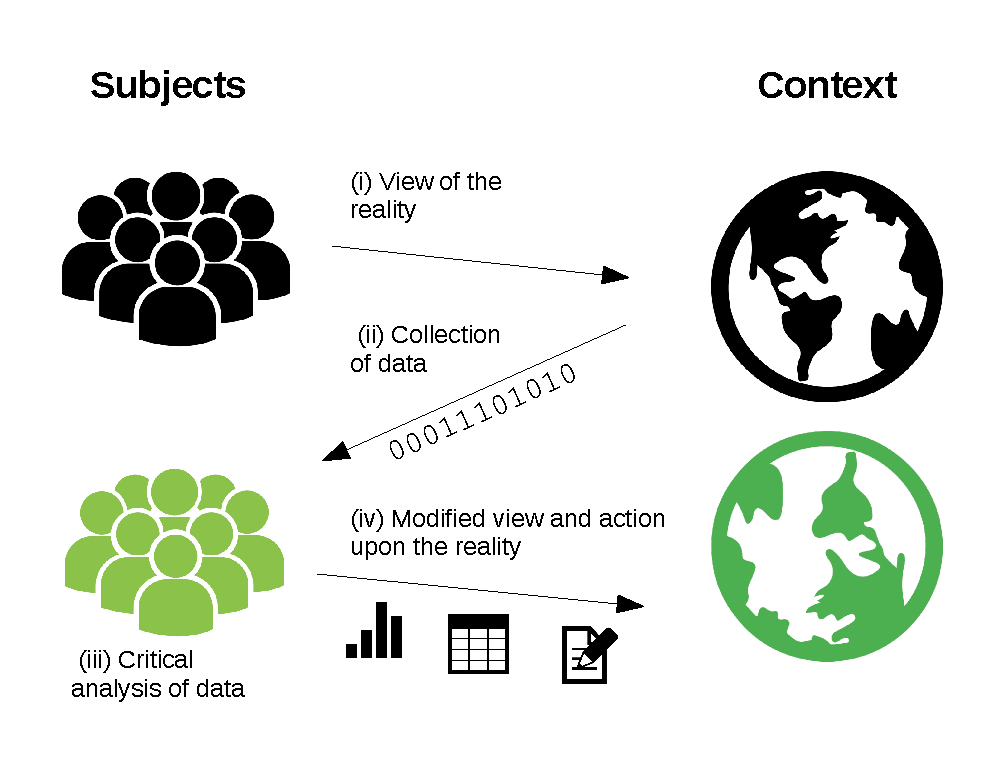
\includegraphics[scale=0.8]{images/critica_data_literacy}
\caption[Critical Data literacy process.]{Critical Data literacy process. Source:~\citeonline{Tygel2015a}}
\label{fig:critical_dl}
\end{center}
\end{figure}

\subsubsection{Data Literacy Stages}

\noindent \textbf{Investigation}

As already stated, this stage must guarantee that the educational process effectively starts from the educands reality. Just like the grape is not a typical fruit from the northeast region of Brazil, a database is also probably not something that is explicitly part of the everyday life of data educands. (Their personal data, however, are almost definitely registered in one or more databases.) At the same time, it is important to seek in the reality of each educand elements where data can be useful to understand that reality. Considering possible problems in dealing with computers, it is fundamental that the themes to be worked with are of great interest of educands, and have their foundations in daily life. It is also important to find contradictions in this reality that one desires to overcome. Thus, an interesting way of starting this quest is through statistics. For example, as detailed in~\citeonline{Tygel2015}, in a data literacy course, the educands were exposed to statistical informations previously selected about their realities. From this point on, it was shown that, on the one hand, datasets were already part of their life, and on the other hand, that much information known by the educands were omitted by data. Thereby, a data mediated world view is approached, facilitating the most adequate choice of thematic axis to work with.

\noindent \textbf{Thematisation}

At this stage, the main goal is to motivate the understanding of the world through data. Either for a local or global reality, about specific or generic themes, data allows an understanding of reality commonly seen as “neutral” or “objective”. At the thematisation stage, it is still possible to keep this aspect, which will be further deconstructed in the problematisation stage.

By elaborating thematic axes, in this stage the aim is to code certain contexts as data and aggregated information, such as statistics, graphics and tables. This coding may lead to more complex decoding about the same theme. A reality can be coded into data, which can be once more coded into aggregated information, and then can be further decoded, generating a modified view over the same reality. It is always important to notice that this process has an intrinsic bias, related to the design choices at data acquisition and processing. 

As a result of this stage, it is possible to obtain the generative themes, which in the case of data literacy, are specific context coded into data. This data can be already available as open databases, closed and subject to information access requests, or may also be uncollected data, which could provide some interesting perspectives. The final aim of this stage is to enchant educands with the world of data that represents realities.

\noindent \textbf{Problematisation}

After the “enchantment” with the world of data, it is fundamental to problematise it, i.e., to unveil what is behind the scenes when talking about data. In order to use data with critical conscience, it is necessary to know where they came from, how and to what purpose they were generated. Thus, it is possible to politicise the use of data, and deal with them not only from the point of view of a passive user, but from the perspective of someone who is also able to produce data, and with them, “say his word”. The final aim of this stage is to promote a critical view about the chosen theme, understanding the role of data for enlightening certain aspects and hide others. We list here, without any aspiration of completeness, two issues that can serve as a starting point for the problematisation stage:

\begin{itemize}
\item \emph{Non-neutrality of Data:} Data are not neutral. The seducing precision and objectivity of data grounded statements almost always hide ideologies and intentions about anything one wants to prove. Thus, it is fundamental to problematise the origin of data. Are data from the government or from civil society organizations? What was the political position of that organization at the time when data were generated? If it is about scientific data, who funded the research? More complex, but also of great importance, is the knowledge of the methodology used to gather data. Lack of awareness of the methodological approach can lead to misunderstandings and flawed conclusions. 

With that information – origin and method – it is possible to infer what was the objective of data generation, where it is not explicit. Producing data is a costly activity, which requires a considerable amount of resources, especially when dealing with big populations and/or wide areas. Therefore, every research that generates data has a very well defined purpose, which must be unveiled and discussed.

Research is designed by specific actors, to reach strategic goals. Similarly, methodologies are designed in order to highlight some aspects, and not others. This is why we can affirm that data resulting from these researches are not neutral, and therefore its non-neutrality must be problematised in a critical perspective of data literacy education.

\item \emph{Transparency:} In many cases, the critical use of data will come across the lack of available data. These missing data may not exist, be hidden or poorly organized, which is the case of many governmental data. In order to work critically with data, it is necessary to have conscience of one's rights to access information, which is directly related to transparency policies. Many countries are advancing in this field, publishing their data online and creating laws to guarantee access to information, transparency and open data, with the valuable argument of enhancing democracy and fighting corruption. However, as stated by the Global Open Data Index, only 11\% of the assessed datasets in 97 countries are open. Thus, discussing transparency and access to information is a possibility of problematising data literacy.  

\end{itemize}

\noindent \textbf{Systematisation}

The systematisation process requires data and information about an experience. In the data literacy context, the ability to put together data retrieved from various external sources with subjective qualitative information empirically obtained should be encouraged.

The systematizing stage should be the conclusion of the whole lived process – investigation, thematisation and problematisation. Of crucial importance is the communication of the results. Data can be exposed in several forms, such as graphics, tables, maps, infographics, music, film or even text. The ability to choose the right way of systematizing and communicating data is certainly a point that should be stressed in data literacy. 

\subsubsection{Definition}

Considering the arguments developed in this section, we derive our definition of critical data literacy:
Critical Data Literacy is the set of abilities which allows one to use and produce data in a critical way. This set is composed by:

\noindent \textbf{Data reading:} \emph{The ability of reading data starts at understanding how data was generated, i.e., which methodologies were used in order to capture data from a context, which facts, measures and dimensions were considered, and at which level of detail, or granularity, data was collected. It also includes understanding who produced it, in which context and why. Data should not be read as objective fact, but as the output of a social process.}

\noindent \textbf{Data processing:} \emph{The ability to technically process data is related to the use of computational and statistical tools in order to transform data into information. Linking data with other sources is also an important skill. Data should be processed based on explicit objectives.}

\noindent \textbf{Data communication:} \emph{The ability to communicate data comprises finding better matches between data types, such as distributions, temporal series, networks or comparisons, and communications tools, such as text, tables, several types of charts, maps or infographics combining these elements. Communicating data also encompasses a social evaluation of what message should be transmitted to which target audience. Data communication should be done in an ethical, responsible and precise way, in order to avoid misunderstandings or invalid conclusions.}

\noindent \textbf{Data production:} \emph{The ability to produce data includes deepening all elements within data reading. Additionally, knowledge about data formats and data publishing tools is required. Generally, data should be published not only respecting the Open Definition, but also offering tools so that non-experts are able to use it.}



\subsection{Conclusions}

The fast spreading of ICTs in the society has, as one of its consequences, a recent publication of massive quantities of data over the Web. These can be either related to governments, through public transparency initiatives, or generated by companies or civil society organizations, or even originated from scientific research. This huge mass of new information brings with it a series of potential benefits, but also major challenges, which are for the most part not as explicit as the benefits. There is an imminent risk of establishing an elite able to profit from these data, interpret it and act in the world through it, while most of the people remain excluded. In this paper, we sought in the work of Paulo Freire inspirations for the construction of a critical data literacy, which incorporates awareness of this challenge.

Future works on this topic includes deriving more tangible examples of the application of this methodology in practice, followed by developing a strategy to assess and evaluate the outcomes. From the theoretical point of view, a deep analysis of the digital literacy literature could also bring more elements for data literacy. 

It was not by accident that Paulo Freire materialized his Popular Education pedagogy into a literacy method. For him, literacy is not only useful to read words, but to read the world. And imbued precisely by this spirit, we propose an analysis of data literacy based on Freire's Literacy Method. By doing so, we hope to provide a small contribution to the democratization of access to information. Data alone do not change the world, but we believe that people who critically understand the reality through data have better tools to do it.

\section[Teaching Open Data for Social Movements: action and research for open data engagement]{Teaching Open Data for Social Movements: action and research for open data engagement\footnote{This section is adapted from~\citeonline{Tygel2015}}}

\label{dl_method} 

Motivated by research on use and publication of open data by social movements and grounded on popular education principles, an open data course was developed. According to the dialogicity principle, the course objective is double: (i) to tackle the issue of open data education, indicated to be one of the factors hindering the use of open data; and (ii) to use the time in training to observe the activists using data and gather information for the research.

The course programme was elaborated seeking a balance between the social aspects of the use of data, the principal motivation, and the technical issues that are inherent in the tools for data manipulation. The methodology switches between expository stages and individual and collective activities by the students. It is expected that the students can at least achieve a critical view about data, understand the possibilities and limits of its use, be aware of the political questions involved in data production and publishing, and, finally, have a technical starting point for manipulating data.

The course is divided into four stages of four hours each, but can be adjusted to needs of the people involved. A website containing teaching materials, links to data sources, and a discussion forum was developed, which in each presentation of the course is supplemented with more data.
Only two requirements are asked of people interested in attending the course: a basic knowledge of informatics (web navigation) and access to a computer (which could also be offered by the organizers). Good quality internet access provided by the organizers is also highly desirable.

\subsection{First Stage – Introduction}

The first stage starts with a short description of the course, and the participants are informed that they will also be contributing to a research project. This stage is intended to get people on the same level, by discussing the sociotechnical and political aspects of data. The aim is to start from the educands' own experience, as suggested by the Popular Education approach. For this, all participants are asked to present themselves, state their expectations and why he or she decided to take part.

Afterwards, a challenge is proposed: some socially relevant statistical results are presented (see Listing~\ref{tab:dl_examples}), and the educands are asked to find the data sources related to those figures. Following the inverse path (information to data, rather than the opposite), we expect to raise curiosity and show, in practice, the importance of knowing what is behind the statistics.

\renewcommand{\arraystretch}{1.8}
\begin{table}[h]
\ABNTEXfontereduzida
\centering
\caption{Examples of data driven statements used to stimulate a critical view of data sources (based on Brazilian statistics agencies)}
\label{tab:dl_examples}
\begin{tabular}{ll}
\hline
\multicolumn{1}{|l|}{1} & \multicolumn{1}{l|}{0.9\% of the biggest landowners own 45\% of arable land in Brazil} \\ \hline
\multicolumn{1}{|l|}{2} & \multicolumn{1}{l|}{\begin{tabular}[c]{@{}l@{}}In Brazil, white men earn more than white women, who earn \\ more than black men, who earn more than black women\end{tabular}} \\ \hline
\multicolumn{1}{|l|}{3} & \multicolumn{1}{l|}{77\% of young people killed in 2011 in Brazil were black} \\ \hline
\multicolumn{1}{|l|}{4} & \multicolumn{1}{l|}{\begin{tabular}[c]{@{}l@{}}46.7\% of Brazilian exportation in 2013 were basic products, \\ 12.6\% were semi- manufactured, and 38.4\% were manufactured\end{tabular}} \\ \hline                                                                                    
\end{tabular}
\end{table}

In the sequel, several open data related topics are discussed:

\noindent \textbf{How does data arise:} a data path is presented, from the occurrence of something, passing through its systematization to its publication. Concepts such as facts, dimensions, and measures are discussed, together with the political motivations and consequences of those design choices. This topic is intended to put data neutrality in question, by showing that data produced by research is an outcome of several choices, made according to some goal.

\noindent \textbf{Data visualization:} the same dataset can be observed in many ways, and the conclusions to which one may come heavily depend on this. Visualizing data as tables, graphics, networks (graphs), or maps may reveal different aspects and induce several kinds of conclusions.

\noindent \textbf{Open Data:} In this topic, we motivate the understanding of open data using analogies (see Table~\ref{tab:open_close}). In the sequel, we define open data according to the David Eaves' three rules: data must by findable in the Web, published in machine readable formats, and cannot have licenses which prevent re-use (Eaves, 2009). A debate about linking and semantically marking data through the use of Linked Open Data (LOD) is also proposed with examples.
Transparency Policy: At this point, we present the context of open data in Brazil and in the world, especially through transparency policies. It starts with the Freedom of Information Act (FoIA), and goes up to Internet governance, with the recent Brazilian regulation1 based on three foundations: net neutrality, privacy and freedom of expression. International efforts on transparency, such as the Open Government Partnership (OGP) are also presented.

\noindent \textbf{Synthesis:} After presenting all topics, educands are asked to discuss how open data is related to their activism.

\begin{table}[]
\centering
\ABNTEXfontereduzida
\caption{Open and closed analogies to help understand what open data is.}
\label{tab:open_close}
\begin{tabular}{|l|l|}
\hline
\multicolumn{1}{|c|}{\textbf{Open}}        & \multicolumn{1}{c|}{\textbf{Closed}}           \\ \hline
Text in digital format (txt, odt, doc)     & Printed Text                                   \\ \hline
Presentation in editable format (odp, ppt) & Presentation in PDF format \\ \hline
Source code                                & Executable software                            \\ \hline
Raw Data                                   & Information (statistics, graphics, maps)       \\ \hline
\end{tabular}
\end{table}

\subsection{Second Stage – Data Sources}

The second stage of the course is dedicated to an overview of some important datasets on the Internet. It is worth noting that some of them are not “open” by the classical definition (Eaves, 2009), mainly because the raw data is not available for download. However, when an aggregate data querying system is offered, it makes data even more useful for common user than if raw data was available.

Different forms of accessing data are discussed. We recognize that, in respect to data access means, there is a trade-off between the ease of analysing data and the autonomy one can have in assessing one’s own conclusions. When a database is published as raw data, following all open data principles, this still might not help a citizen who wants to know how much was spent on education is his city. Large volumes of data coded in specialized formats (e.g. R, SPSS, SAS, SQL, XML, RDF) allow a high level of autonomy in the analysis, but special skills are needed to work with it. On the contrary, aggregate data, reports and charts allow people to have access to this information, but it has already passed through someone else's filter. Figure 1 depicts this debate. 

\begin{figure}[h!]
\begin{center}
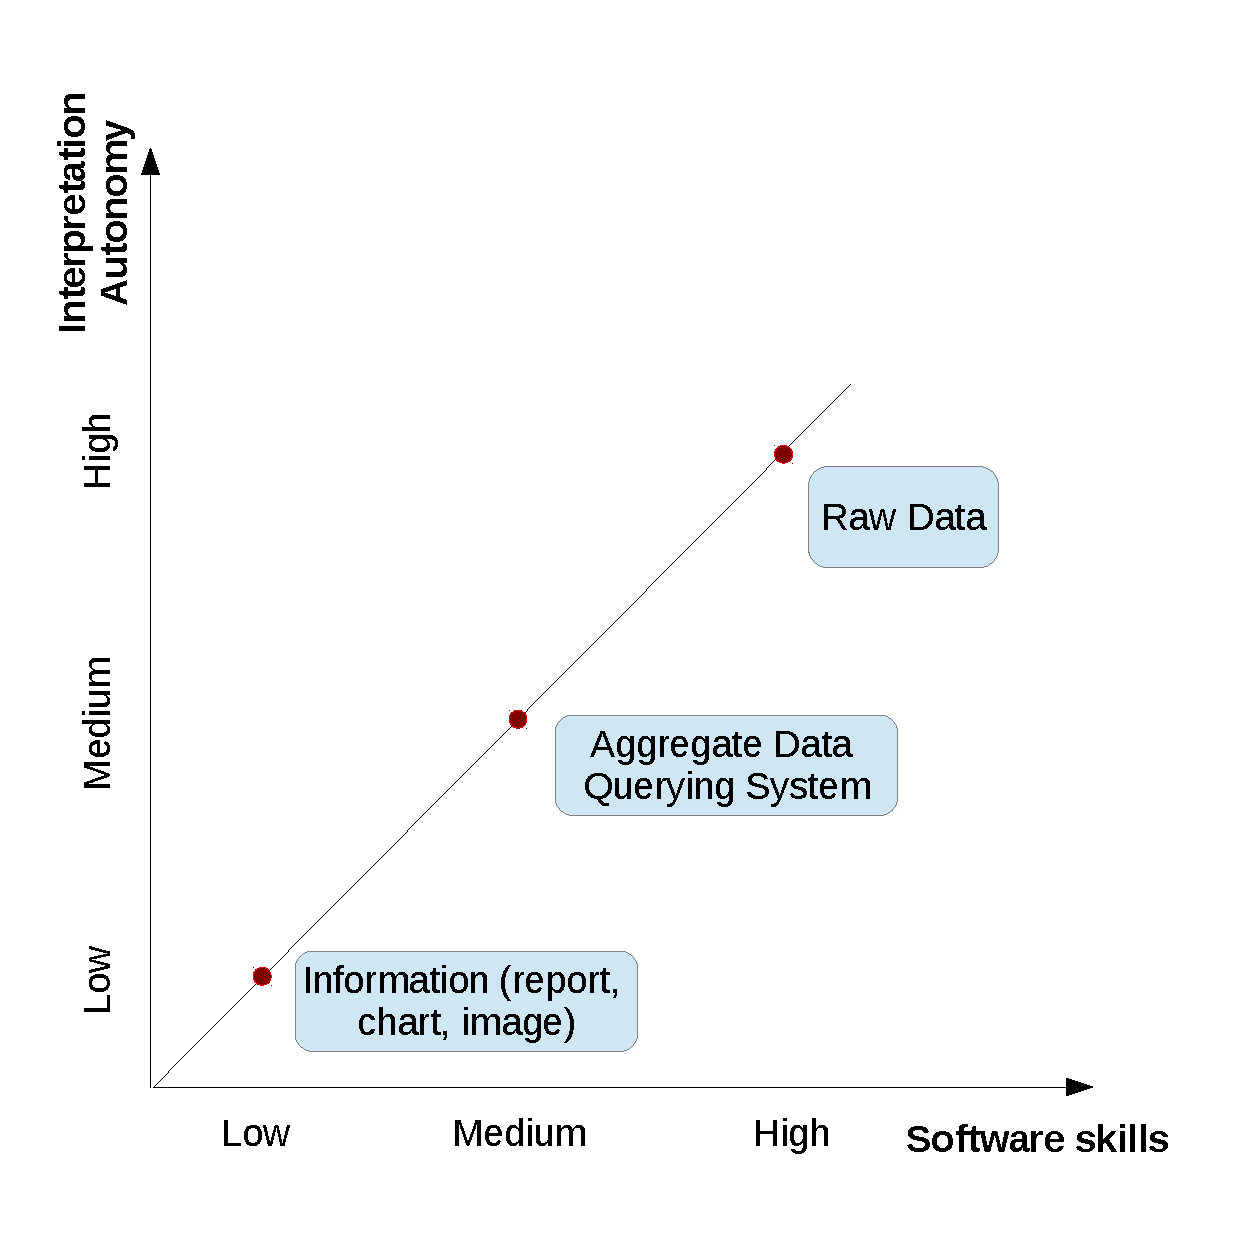
\includegraphics[scale=0.6]{images/opendatatradeoff.pdf}
\caption{Trade-off between interpretation autonomy and software skills needed.}
\label{fig:opendatatradeoff}
\end{center}
\end{figure}

Besides the means of data access, we propose a classification of data according to the type of provider:
Data produced by the state: This is the wider category, since the state has structural conditions and legal liability to produce data. In Brazil, the biggest data producer is the Brazilian Institute of Geography and Statistics (IBGE, in Portuguese), responsible for demographic, economic, geographic and many other sorts of data. The Unified Health System (SUS, in Portuguese) is also an important data generator, mostly about health and illnesses. Worldwide, the United Nations (UN) and the World Bank are also important data suppliers. Even though they are not governments, most of their data is compiled from country data. It is important to emphasize that this kind of data carries with it the visions and ideologies of those who generated it. All the design choices made during the data production, including definition of facts, dimensions, and measures, in some degree follows the government intentions.

Data produced by the state and shown by society: In many cases, data produced by the state is not open, and when it is open, there are no tools for the citizens to easily analyse and take their own conclusions. Specialists are needed in order to translate data into useful information. In order to tackle this issue, many society-driven applications using official data have been recently released. In many cases, they help visualize data in a way that leads to conclusions against the states' interest. One example is the Brazilian's “Congress Owners” application. Based on raw (and hard to analyse) donation data published by Electoral Justice, a civil society organization has developed an application where people can easily access and visualize the amount of donations received by politicians and parties, or paid by enterprises or economic sector. 

Data produced by society: The case where organized groups of the civil society produce their own data is interesting because: (i) as in the case of state data, data produced by the civil society contains its ideological influences in the design choices; (ii) it allows other perspectives on subjects already explained by the state. 

Data related stories can oppose well established hegemonic opinions. One example is the Brazilian Map of Environmental Injustice. Agribusiness is considered to be a good development alternative for the country, based on its relevant contribution to the gross domestic product. The map shows 82 occurrences of Environmental Injustice related to the agribusiness (from a total of 501), where activities of this sector cause damage to poor communities and/or to the natural habitat. Table~\ref{tab:sm_initiatives} shows a number of society driven databases. It is worth noting that, in some cases, the funding for building those databases comes from the Government. In principle, we consider that this does not hurt society’s autonomy and freedom to put their views forward in the design process.


\begin{table}[]
\centering
\ABNTEXfontereduzida
\caption{Examples of society driven databases, used by social movements with several purposes.}
\label{tab:sm_initiatives}
\begin{tabular}{|l|l|}
\hline
\multicolumn{1}{|c|}{\textbf{Initiative}}  & \multicolumn{1}{c|}{\textbf{Publisher}}  \\ \hline
\begin{tabular}[c]{@{}l@{}}\href{http://www.conflitoambiental.icict.fiocruz.br/}{Environmental} \\ Injustice Maps\\  (Brazil)\end{tabular} & Fiocruz and FASE                                                                                                                            \\ \hline
\begin{tabular}[c]{@{}l@{}} \href{http://conflitosambientaismg.lcc.ufmg.br/}{Environmental} \\ Conflicts Maps \\ (Minas Gerais, \\ BR)\end{tabular}       & \begin{tabular}[c]{@{}l@{}}Federal University of Minas Gerais, \\ Brazil (in partnership with a number \\ of social movements)\end{tabular} \\ \hline
\begin{tabular}[c]{@{}l@{}} \href{http://www.ejolt.org/maps/}{Atlas of} \\ Environmental \\ Justice\end{tabular} & \begin{tabular}[c]{@{}l@{}}23 worldwide organizations (see \\ http://www.ejolt.org/section/team \\ for a complete list)\end{tabular}        \\ \hline

\href{http://agroecologiaemrede.org.br}{Agroecology initiatives}  & \begin{tabular}[c]{@{}l@{}}ANA/ABA (Brazilian national social \\ movements related to agroecology)\end{tabular}                             \\ \hline
\href{http://cptnacional.org.br/}{Land Conflicts} & Comissão Pastoral da Terra (CPT)                                                                                                            \\ \hline
\end{tabular}
\end{table}

In the final activity of this stage, educands are asked to add new data sources to the course web page, according to their interests. New sources can come from students' experiences, or be searched for during the class time. However, it is important to find the exact link, since this is reported to be a difficulty, as it will be seen later.

\subsection{Third Stage – Tools}

In the third stage, the focus is on tools for manipulating data. The goal is to present the means to work with the raw or aggregate data resulting from queries. It begins with an introduction to the Comma Separated Values (CSV) format, which is an open, universal and easy-to-use way of exchanging tabular data. Concepts such as primary and foreign keys are also discussed, in order to help comprehend how relationship between tables and databases can be made. Nevertheless, database design is beyond our scope.

This is an essentially practical stage. Several tools are presented, so that each student can choose which one he or she wants to work with, according to individual interests and ability with computers.

The first tool presented is a spreadsheet editor. The task consists in downloading a CSV sheet with a two dimensional table (production of food in tons, by type of food and year) and drawing a line chart. Students are also asked to plot percentage changes between first and last year production. The second part of the task consists in working with dynamic tables, which allows building analysis frameworks with more than two dimensions.

Other tools presented are related to map building and infographics drawing. Sometimes a mathematical background revision is necessary, since working with number variations requires some previous knowledge of percentages.

\subsection{Fourth Stage – Final Work}

The fourth and final stage is dedicated to a jointly decided activity. The goal is to develop some data based communication product, based on the three previous stages. Ideally, there should be more than one facilitator in the room, so that the work can be divided into groups, with each group being accompanied by one instructor.

Suggested options include: writing news text based on data, and building infographics and maps on specific subjects. The intentionality – what and why we want to communicate – is discussed first. Then, we evaluate the feasibility of the task – is there data about this subject? – and finally, the communication instrument is chosen. In the end, results are presented and an evaluation of the course is done.

The next section brings an analysis of presentations of this course, and draws out some research results based on the experiences gained.

\section[Open Data Clues from the Field]{Open Data Clues from the Field\footnote{This section is adapted from~\citeonline{Tygel2015}}}

\label{dl_results} 

In this section, we describe the application and the systematized results of the above detailed open data course.

The course was presented five times in the second semester of 2014, in Brazil. While three presentations happened in Rio de Janeiro, one was held in Vitória (state of Espírito Santo) and another in Porto Alegre (state of Rio Grande do Sul). Two presentations were held in a workers union and three in universities, organized by groups who work with social movements in extension projects. A total of 52 students enrolled and participated in at least one stage. There were no fees to pay, and the only requirements were basic informatics knowledge and access to a computer, sometimes provided by the organizers. Table~\ref{tab:dl_summary} shows a summary of the presentations.

\begin{table}[]
\centering
\ABNTEXfontereduzida
\caption{Summary of the presentations of the open data course for social movements.}
\label{tab:dl_summary}
\begin{tabular}{|l|l|l|l|l|l|}
\hline
\textbf{N.} & \textbf{\begin{tabular}[c]{@{}l@{}}Kind of \\ Place\end{tabular}} & \textbf{City}                                             & \textbf{\begin{tabular}[c]{@{}l@{}}Duration (h) and time\\ distribution\end{tabular}} & \textbf{\begin{tabular}[c]{@{}l@{}}Participants\\ enrolled\end{tabular}} & \textbf{\begin{tabular}[c]{@{}l@{}}Forms\\ responded\end{tabular}} \\ \hline
1           & Union                                                             & \begin{tabular}[c]{@{}l@{}}Rio de \\ Janeiro\end{tabular} & 16h (four days at night)                                                              & 6                                                                        & 2                                                                  \\ \hline
2           & University                                                        & \begin{tabular}[c]{@{}l@{}}Rio de \\ Janeiro\end{tabular} & 16h (two full days)                                                                   & 11                                                                       & 3                                                                  \\ \hline
3           & University                                                        & Vitória                                                   & 16h (four days at night)                                                              & 13                                                                       & 4                                                                  \\ \hline
4           & University                                                        & \begin{tabular}[c]{@{}l@{}}Porto \\ Alegre\end{tabular}   & \begin{tabular}[c]{@{}l@{}}12h (one half day/one \\ full day)\end{tabular}            & 12                                                                       & 3                                                                  \\ \hline
5           & Union                                                             & \begin{tabular}[c]{@{}l@{}}Rio de \\ Janeiro\end{tabular} & 8h (two days at night)                                                                & 10                                                                       & 3                                                                  \\ \hline
\multicolumn{3}{|l|}{\textbf{Total}}                                                                                                        & \textbf{68 h}                                                                         & \textbf{52}                                                              & \textbf{15}                                                        \\ \hline
\end{tabular}
\end{table}
The analysis will be based on two instruments: an evaluation questionnaire that all students were asked to fill in, and a participant observation gathered during the presentations. The goal of the analysis is to respond to the research questions: (i) why social movements use data (motivations); (ii) what are the mains problems (impediments); and (iii) what could be done to enhance the use (improvements). Also, the evaluations about the course can be used to improve it.

\subsection{Questionnaire based analysis}

All the participants were requested to answer a questionnaire after attending the course. Thus, we assume that the opinions given are strongly influenced by the discussions held over the course. This decision was taken having in mind that: (i) open data is not a subject of the educands' everyday life; so, answering before the course could lead to meaningless results; (ii) according to the popular education methods, we expect each educand to be able to relate content unseen before with their experiences, and in the end to synthesize their own conclusions about the process. Table~\ref{tab:questions} shows the questionnaire and the mean, maximum, and minimum values for numerical questions.

\begin{table}[]
\centering
\ABNTEXfontereduzida
\caption[Questionnaire answered by course attendants.]{Questionnaire answered by course attendants. All the numerical results are in over a base of 15 (n = 15), and N/A means “not applicable”.}
\label{tab:questions}
\begin{tabular}{|l|l|c|}
\hline
\multicolumn{1}{|c|}{\textbf{\#}} & \multicolumn{1}{c|}{\textbf{Question}}                                                                                                   & \textbf{\begin{tabular}[c]{@{}c@{}}Mean \\ (maximum \\ - minimum)\end{tabular}} \\ \hline
1                                 & Age                                                                                                                                      & 31 (25–48)                                                                      \\ \hline
2                                 & Knowledge of informatics (1: poor knowledge – 5: good knowledge)                                                                         & 2.7 (1–5)                                                                       \\ \hline
3                                 & Work/Profession/Activism                                                                                                                 & N/A                                                                             \\ \hline
4                                 & \begin{tabular}[c]{@{}l@{}}Why have you attended to the course? Why do you think open data \\ is important?\end{tabular}                 & N/A                                                                             \\ \hline
5                                 & \begin{tabular}[c]{@{}l@{}}Educator's performance (didactics, material, knowledge, punctuality) \\ (1: poor – 5: very good)\end{tabular} & 4.5 (3–5)                                                                       \\ \hline
6                                 & \begin{tabular}[c]{@{}l@{}}Self performance (participation, attention, punctuality) (1: poor – 5: \\ very good)\end{tabular}             & 3.3 (1–4)                                                                       \\ \hline
7                                 & \begin{tabular}[c]{@{}l@{}}Was the subject according to your expectations? (1: totally distinct – \\ 5: totally according)\end{tabular}  & 4.6 (2–5)                                                                       \\ \hline
8                                 & What is the main impediment perceived by using data?                                                                                     & N/A                                                                             \\ \hline
9                                 & How do you imagine that the use of data could be improved?                                                                               & N/A                                                                             \\ \hline
\end{tabular}
\end{table}
The median age of participants was 31 years, with the youngest being 25 years old and  the oldest 48. They considered themselves to have medium knowledge of informatics. Before enrolling, participants were asked to have some informatics knowledge, but no admission tests were given.

Some participants were exclusively activists or academics, but most of them were activists with some academic involvement. There were journalists, lawyers and social scientists, all engaged with some social movement. No participant had formal informatics training, meaning that no one was an informatics expert.

The teacher's performance was well rated, but this was somehow expected in a free course. On the other hand, no one rated him or herself with very good participation performance. In Question 7, only one participant seemed to have very different expectations about the course content. All the others marked 4 or 5, indicating that open data is not so distant from non-informatics people's lives, at least for those who answered the questionnaire.

In order to analyse questions 4, 8 and 9, we will pick answer elements and classify them according to research 
goals: motivations, impediments, and improvements. Question 4 was aimed to catch motivations, but impediments and improvements were also cited. Question 8 raised only impediments, and Question 9 only improvements, as intended.
An effort was made to extract concrete elements from the discursive text. An equilibrium was sought between merging similar statements and not losing the diversity of opinion. These concrete elements extracted can be seen in the Appendix, in Tables~\ref{tab:dl_results1}, \ref{tab:dl_results2}, and \ref{tab:dl_results3}.

Sometimes, the separation between the classes is not very clear. All impediments (e.g. “Open Data Portal is hard to use”) have implicit improvements (e.g. “Open Data Portal could improve usability”), as all improvements also have implicit impediments. Some motivations (e.g. “Use spending data to fight corruption”) also could be interpreted as impediments (e.g. “Few spending data is available”) or improvements (e.g. “More spending data must be made available”). We tried to classify according to the respondent's intention.

\subsection{Observation based analysis}

In this section, some remarks are made based on the 68 hours observation of the course. This observation was driven inspired by the ethnographic method of participant observation~\cite{Atkinson1994}. Within this approach, the researcher plays an established participant role in the studied scene, in this case, as an educator, taking field notes during the class. Ethnography inspired methods are complementary to objective and quantitative evaluations since, according to~\citeonline{Atkinson1994}, ethnography deals with the “analysis of data that involves explicit interpretation of the meanings and functions of human actions”, and “represents a uniquely humanistic, interpretive approach, as opposed to supposedly 'scientific' and 'positivist' positions.” Since two of our research questions deal with human actions and feelings – what are the motivations of social movements for using open data and what are impediments that block a wider and better use – we considered the participant observation an appropriate methodological direction. We aimed to comprehend the point of view of the educands, and this was done from the educator stance, which certainly influenced the analysis.

As described earlier, in the first stages of the course participants are shown statistical statements (see Table~\ref{tab:dl_examples}) and are asked to search for data that generated those figures. Below, we list some behaviours observed:

\begin{itemize}
\item The first impulse of users is to paste the phrases directly into a web search engine. Normally, the results are news commenting that statement, or reports containing that information, and never the actual data source.
\item For some people, it is difficult to understand the difference between the statements and the data sources from which they were originated. One way to overcome this misunderstanding is to slightly rephrase the statement and ask what would be the new figures. For example, relating to statement 1 (Listing 1), we would ask: “how much land do the 0.1\% of the biggest landowners possess?”.
\item Overall, only few people reached the actual data source. This shows that one of the main problems of data sets and their query/download systems is that they are frequently hidden in the deep web, i.e., regular search machines cannot find them.
\end{itemize}

In the second stage of the course, some data sources are presented and divided into three categories. About this stage, we would like to remark:

\begin{itemize}
\item In general, although interested, users are unfamiliar or unaware of data sources. This ignorance is, as expected, worse for society driven OGD based applications, and for data produced by social movements, which usually have no official means of dissemination;
\item Students were stimulated to add new data sources to the course website, according to their own interests or activism. In some cases, participants inserted already known data sources, but in most cases data sources were found during the activity.
\end{itemize}

The third practical stage revealed one of the strongest difficulties in open data usage: the manipulation of software tools, particularly of spreadsheets. The knowledge about CSV tabular files, considered as a fundamental skill to use data on different systems, was practically absent. This problem got even worse because of the inability of the most-used proprietary spreadsheet application (MS Excel) to deal with such kind of file. LibreOffice, its open source counterpart, facilitates this task.

Another issue that was highlighted at this stage was the mathematical difficulty faced by most of the students. Dealing with statistical open data requires, most of the time, simple mathematical operations. Therefore, sometimes a small revision of percentage was necessary.

Unfortunately, the fourth stage of the course did not work as expected. This stage was only reached in two of the five presentations described in Table~\ref{tab:dl_summary}. In the first one, students, mainly journalists, decided to individually write stories and impressions about open data. They were published in the course website. The second experience reached closer to the goal: participants decided to investigate a local case of environmental injustice. Data about enterprises, population health, environmental licensing and other issues were gathered, but no final product was obtained. In the remaining three presentations, the time ran over twice, and once the students said they were tired, as this course was run on two full days, at a weekend.

One possible way to overcome this issue is to propose this work at the beginning of the course and organize tasks during the other stages. This has the advantage of motivating students with a concrete problem during the course. Nevertheless, the challenge remains: how to prepare the course without predefining the problem. Another option would be to increase the number of hours, which would depend on participants' availability.

\subsection{Synthesis}

As explained above, by a simple rephrasing, an impediment or a motivation can turn into an improvement. By doing a careful analysis of Tables~\ref{tab:dl_results1}, \ref{tab:dl_results2}, and \ref{tab:dl_results3} (see the Appendix), an improvement classification tree was built. It is aimed at orienting actions for the engagement of social movements in open data in the Brazilian context. The classification tree can be seen in Figure~\ref{fig:dl_results}.

\begin{figure}[h!]
\begin{center}
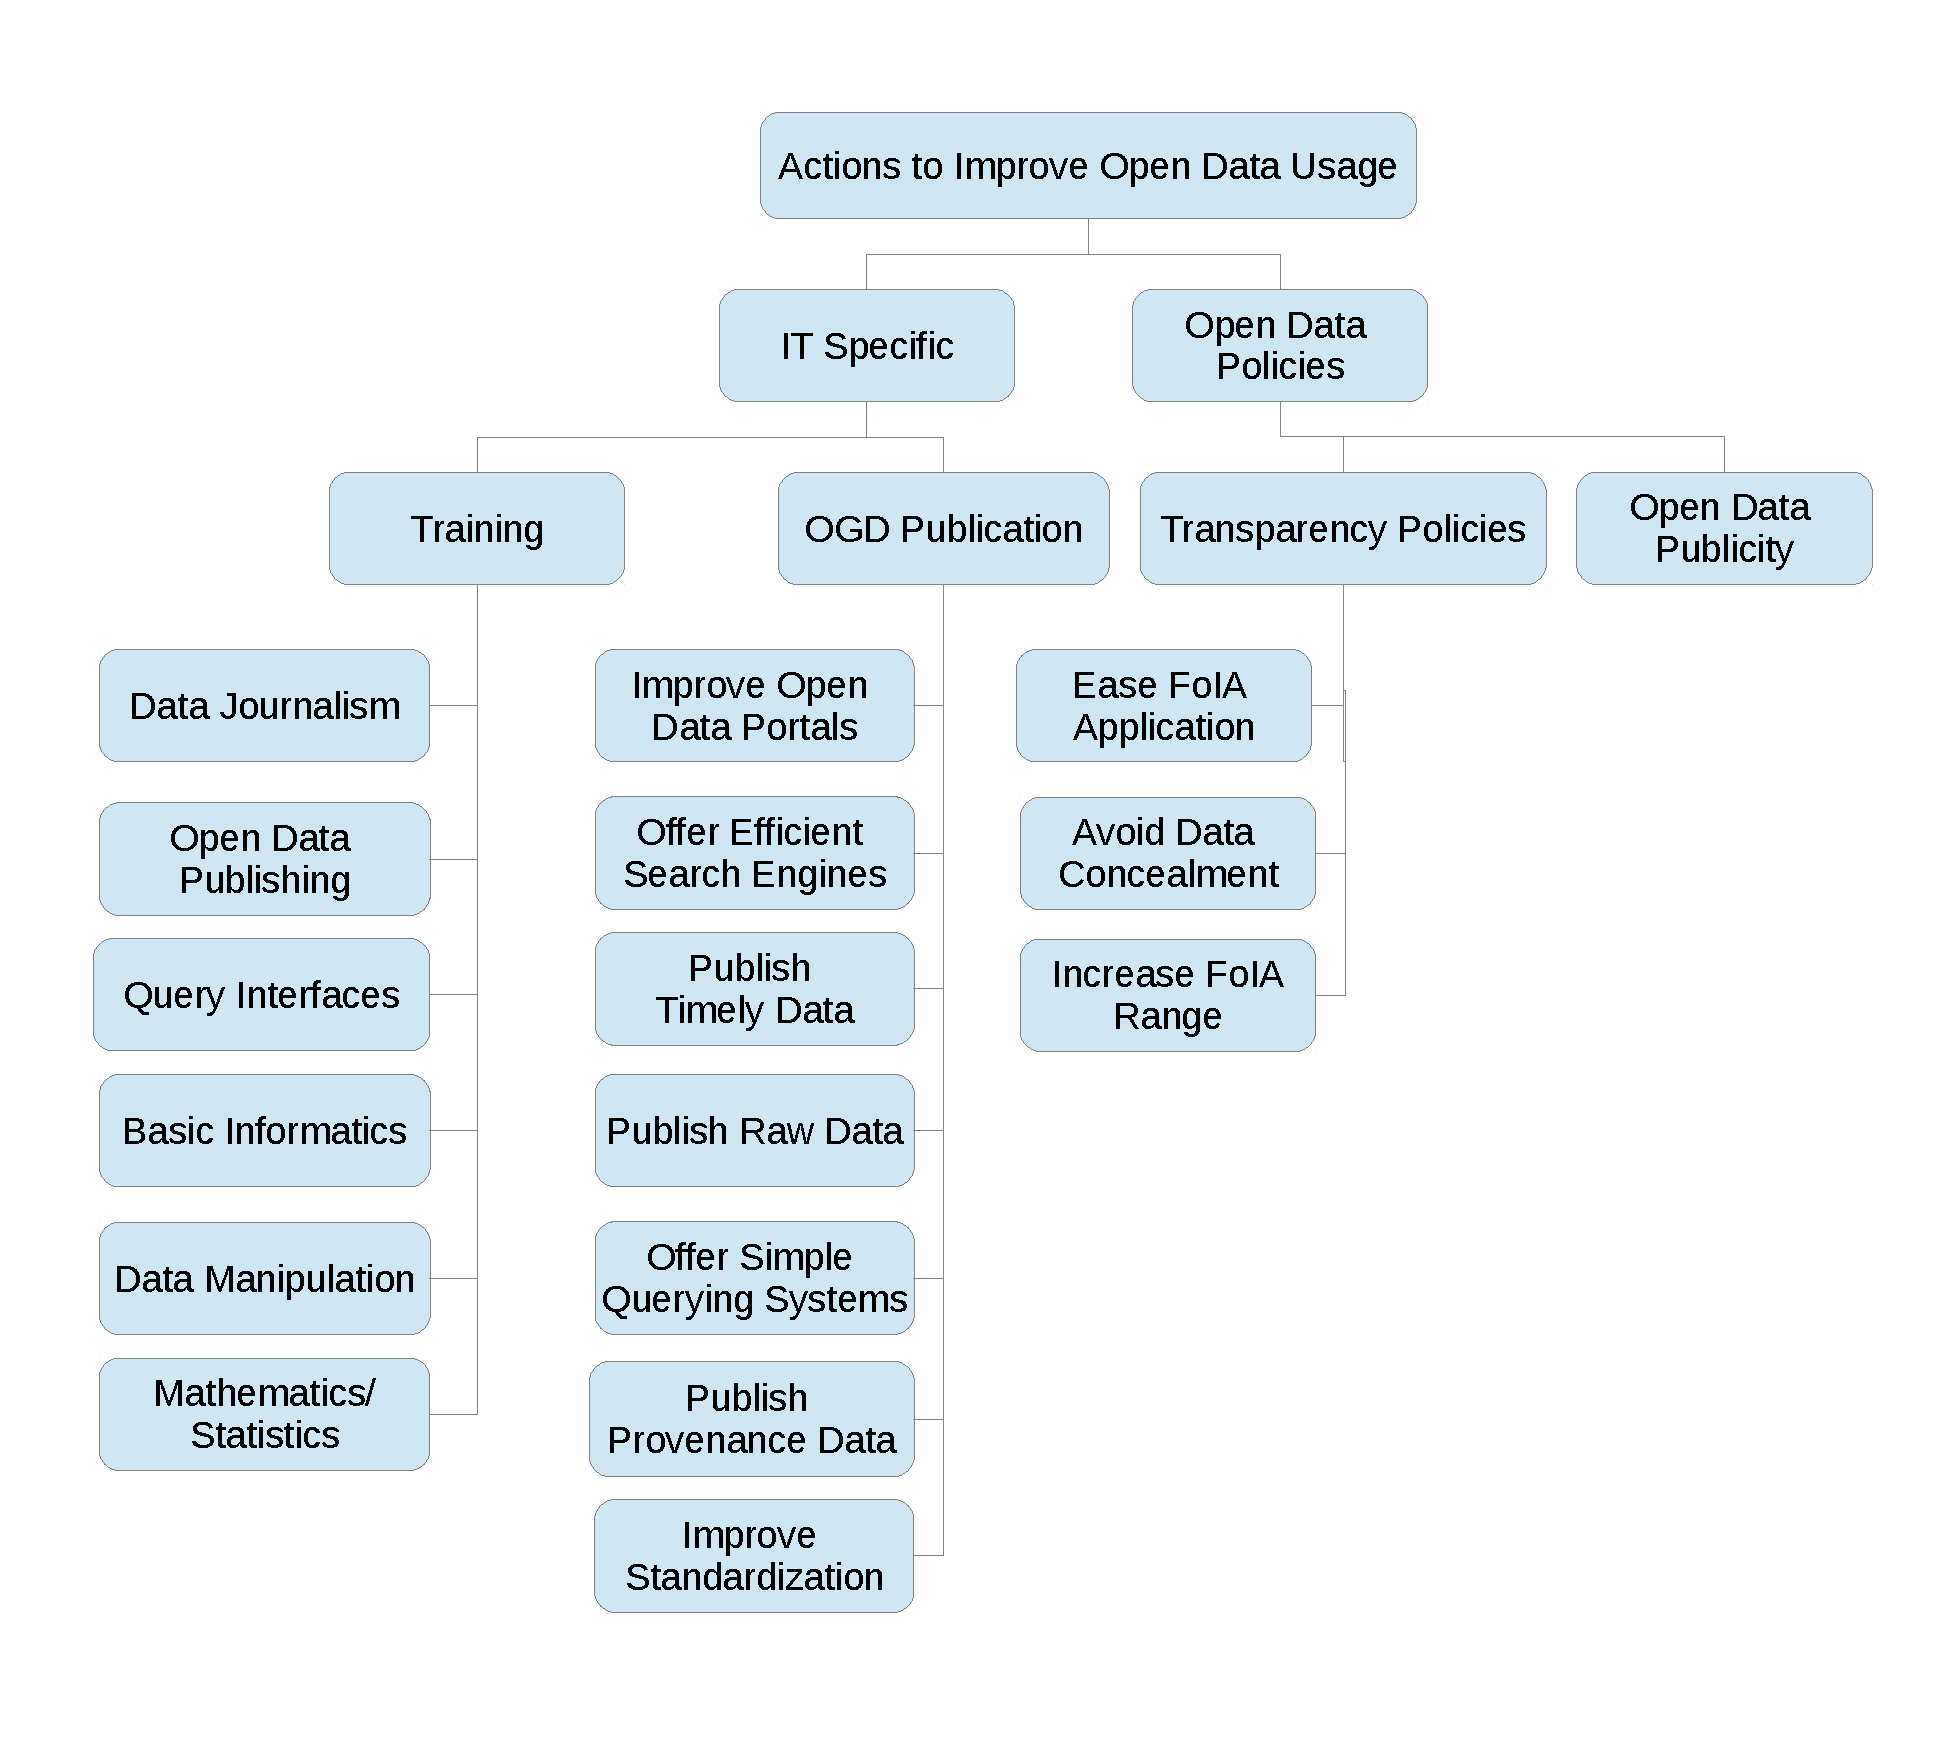
\includegraphics[scale=0.5]{images/impediments_classification.pdf}
\caption[Classification tree for open data engagement actions.]{Classification tree for open data engagement actions, systematized from Tables 6, 7 and 8.
The first classification is a distinction between Information Technologies (IT) Specific and Open Data Policies related issues. There is no intention to imply a duality between social and technical issues, however, one can easily recognize that some elements are directly related to information technology, and others are not.
}
\label{fig:dl_results}
\end{center}
\end{figure}


The IT Specific issues are divided into Training and Open Government Data (OGD) Publication. The first class encompasses cited impediments which could be approached with educational investments, and the second is related to actions to be taken by government data publishers. Our proposed course tackles all cited educational demands, except data publishing, since it still demands a higher level of informatics knowledge.  As to OGD Publication related issues, the need for better search engines was the most cited enhancement.

The right side of the tree presents general issues related to Transparency Policies and Open Data Publicity. We can conclude that in order to improve open data usage, actions must be taken far above data level. In this case, the whole structure for information access must be enhanced. Difficulties in claiming the FoIA within local government levels were reported, as well as accessing information on private foundations that run on public money. Finally, many participants suggested that more publicity on open data already available would also improve usage.

%\subsection{Comments}

%This section described a methodological strategy used in research on Open Data and Social Movements. An open data course was proposed in order to help understand the motivations for the use of open data by social movements, the impediments to succeed with this, and the improvements that could help the engagement of society by means of open data.

%The results of five presentations of the course were organized into a classification tree of possible open data engagement actions, shown in Figure 2. Training related actions should be fostered as part of a Transparency Policy, but social movements should also prioritize open data in their agenda.

Some improvements related to OGD publication could be addressed by using new technologies being developed under the Linked Open Data (LOD) framework. By semantically annotating data with commonly used vocabularies and ontologies, the LOD approach offers the technical means to link different data sources and jointly query them. A solid set of tools to implement LOD is being developed~\cite{Auer2014}, but strong efforts must be made to hide the complexity of the representation and to highlight its benefits, so that it can be recognised as a viable option. Other improvements are only possible through the effective political willingness of governments to be transparent.

As a methodological approach for research in informatics, the course was found to be an efficient tool, since it accomplished its dialogical function indicated by the Popular Education theory. At the same time as they were subjects on an open data education action, the educands that participated on the course acted as objects in a research project. On one side the dialogical approach resulted in a set of appointments for open data publishers; on the other side, in a satisfactory educational experience, as shown by the good educator evaluation (Table~\ref{tab:questions}) and by the rich answers collected (Tables~\ref{tab:dl_results1}, \ref{tab:dl_results2}, and \ref{tab:dl_results3}).

%The open data engagement actions gathered here are not supposed to be complete. The methodology used to raise these actions allows only to affirm that they can improve the use of a specific actor, a social movement, that thinks about open data with a special intentionality. Nevertheless, our efforts add to a number of other initiatives~\cite{Atz2015, Davies2013,Gurstein2011, Ubaldi2013, Veljkovic2014, Zuiderwijk2014}, encompassing other actors, and aiming to picture a desired open data scenario in the future.

\section{Conclusion}
\label{dl_conclusion} 

In this chapter, we presented both a participatory research on open data and theoretical and practical contributions to data literacy.
Together with the open data landscape presented in the previous chapter, we formed a solid view over the question dealt in this thesis. 
Considering that open data organization is an important question that hinders the achievement of open data promises, in the next chapters we will present a related approach.
The following chapter presents a literature review on methods for dealing with semantic metadata, and is followed by Chapter~\ref{chap:tagging}, where we present the Semantic Tags for Open Data -- STODaP -- approach.

